% Created 2021-12-27 lun 10:50
% Intended LaTeX compiler: pdflatex
\documentclass[conference]{IEEEtran}
\usepackage[utf8]{inputenc}
\usepackage[T1]{fontenc}
\usepackage{graphicx}
\usepackage{longtable}
\usepackage{wrapfig}
\usepackage{rotating}
\usepackage[normalem]{ulem}
\usepackage{amsmath}
\usepackage{amssymb}
\usepackage{capt-of}
\usepackage{hyperref}
\input{~/org/latex/author_TeoCir2_Riedinger.tex}
\input{~/org/latex/ieee.tex}
\date{\today}
\title{Diseño de filtros digitales TIIR basados en el microcontrolador STM32F429ZI}
\hypersetup{
 pdfauthor={},
 pdftitle={Diseño de filtros digitales TIIR basados en el microcontrolador STM32F429ZI},
 pdfkeywords={},
 pdfsubject={},
 pdfcreator={Emacs 27.2 (Org mode 9.6)}, 
 pdflang={Spanish}}
\begin{document}

\maketitle
\tableofcontents


\section{Introducción:}
\label{sec:org002bdce}

Un filtro es un sistema, que dependiendo de algunos parámetros, realiza un proceso de discriminación de una señal de entrada obteniendo  variaciones en su salida. Los filtros digitales tienen como entrada una señal digital y a su salida tienen otra señal digital, pudiendo haber cambiado en amplitud, frecuencia o fase dependiendo de las características del filtro.

El filtrado digital es parte del procesado de señal digital. Se le da la denominación de digital más por su funcionamiento interno que por su dependencia del tipo de señal a filtrar, así podríamos llamar filtro digital tanto a un filtro que realiza el procesado de señales digitales como a otro que lo haga de señales analógicas.

El filtrado digital consiste en la realización interna de un procesado de datos de entrada. El valor de la muestra de la entrada actual y algunas muestras anteriores (que previamente habían sido almacenadas) son multiplicadas, por unos coeficientes definidos. También podría tomar valores de la salida en instantes pasados y multiplicarlos por otros coeficientes. Finalmente todos los resultados de todas estas multiplicaciones son sumados, dando una salida para el instante actual. Esto implica que internamente tanto la salida como la entrada del filtro serán digitales, por lo que puede ser necesario una conversión analógico‐digital o digital‐analógico para uso de filtros digitales en señales analógicas.

Los filtros digitales se usan frecuentemente para tratamiento digital de la imagen o para tratamiento del sonido digital.

\subsection{Tipos de filtros:}
\label{sec:orgb25199a}

Hay varios tipos de filtros así como distintas clasificaciones para estos filtros:

\begin{itemize}
\item De acuerdo con la parte del espectro que dejan pasar y atenúan hay:

\begin{itemize}
\item Filtros pasa alto.
\item Filtros pasa bajo.
\item Filtros pasa banda.
\begin{itemize}
\item Banda eliminada.
\item Multibanda.
\item Pasa todo.
\item Resonador.
\item Oscilador.
\item Filtro peine (Comb filter).
\item Filtro ranura o filtro rechaza banda (Notch filter).
\end{itemize}
\end{itemize}

\item De acuerdo con su orden:

\begin{itemize}
\item Primer orden.
\item Segundo orden o superior.
\end{itemize}

\item De acuerdo con el tipo de respuesta ante la entrada unitaria:

\begin{itemize}
\item FIR (Respuesta Finita al Impulso o \emph{Finite Impulse Response}).
\item IIR (Respuesta Infinita al Impulso o \emph{Infinite Impulse Response}).
\item TIIR (Respuesta Infinita Truncada al Impulso o \emph{Truncated Infinite Impulse Response}).
\end{itemize}

\item De acuerdo con la estructura con que se implementa:

\begin{itemize}
\item Directa.
\item Transpuesta.
\item Cascada.
\item Fase lineal.
\item Laticce.
\end{itemize}
\end{itemize}

\subsection{Expresión general de un filtro digital:}
\label{sec:org885f7ba}

En muchas aplicaciones del procesado de señales es necesario diseñar dispositivos o algoritmos que realicen operaciones sobre las señales y que los englobaremos bajo la denominación genérica de sistemas.

Un sistema opera sobre una señal de entrada o excitación según una regla preestablecida, para generar otra señal llamada salida o respuesta del sistema a la  excitación propuesta y que puede simbolizarse:

\begin{equation}
    y[n] = T(x[n])
\end{equation}

donde \(T\) simboliza la transformación, operador o procesado realizado por el sistema sobre la señal \(x\) para producir la señal \(y\) (ver Fig. \ref{fig:esquemaFiltro}). Una de las motivaciones más fuertes para el desarrollo de herramientas generales para el análisis y diseño de sistemas es que proviniendo a menudo de aplicaciones muy diferentes tienen descripciones matemáticas similares.

\begin{figure}[htbp]
\centering
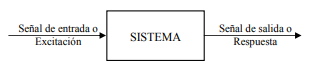
\includegraphics[width=.9\linewidth]{../images/esquemaFiltro.png}
\caption{\label{fig:esquemaFiltro}Esquema de sistema, señal de entrada y respuesta o salida del sistema}
\end{figure}

Existen varias maneras de representar un sistema, ya que muchos sistemas reales están construidos como interconexiones de varios subsistemas, tal como se grafica en la Fig. \ref{fig:interconexionSistema}.

\begin{figure}[htbp]
\centering
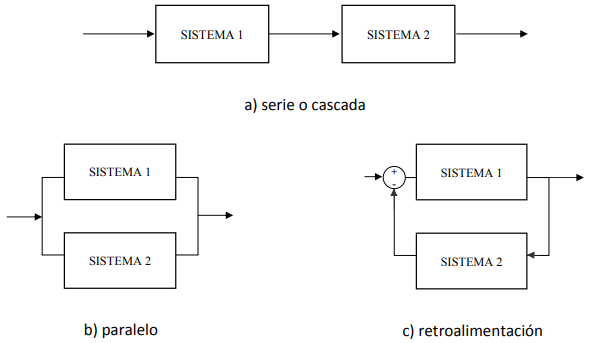
\includegraphics[width=.9\linewidth]{../images/interconexionSistema.png}
\caption{\label{fig:interconexionSistema}Interconexión de sistemas}
\end{figure}

Existen dos métodos básicos para el análisis del comportamiento o respuesta de un sistema lineal a una determinada entrada. Un primer camino se basa en obtener la solución de la ecuación entrada‐salida del sistema que en general tiene la forma de las ecuaciones en diferencias lineales a coeficientes constantes \(a_{m}\), \(b_k\):

\begin{equation}
    \sum_{m=0}^{N_a - 1}{a_m y[n-m]} = \sum_{k=0}^{N_b - 1}{b_k x[n-k]}
    \label{eq:defFiltro}
\end{equation}

siendo \(N_a\) y \(N_b\) los órdenes máximos de las diferencias en la ecuación correspondiente a la entrada y a la saldia del sistema.

El segundo método para el análisis del comportamiento del sistema reside en la aplicación del principio de superposición y consiste en descomponer la señal de entrada en una suma pesada de señales elementales las cuales se escogen de manera que sea conocida la respuesta del sistema a las mismas. Siguiendo esta línea, una señal a tiempo discreto puede visualizarse como una secuencia pesada de impulsos unitarios:

\begin{equation}
    x[n] = \sum_{k=-\infty}^{\infty}{x[k] \cdot \delta [n - k] }
\end{equation}

Aplicando la propiedad de superposición de los SLIT (Sistemas Lineales e Invariantes en el Tiempo) (Oppenheim y Willsky, 1983), se puede determinar la salida del sistema ante una cierta entrada de la siguiente manera:

\begin{equation}
    y[n] = \sum_{k=-\infty}^{\infty}{x[k] \cdot h[n-k]}
\end{equation}

siendo \(h[n]\) la respuesta o salida del sistema ante una entrada equivalente a un impulso unitario \(\delta [n]\) denominada \emph{respuesta al impulso del sistema}. El segundo miembro de la expresión representa el producto de convolución de la señal de entrada \(x[n]\) y la respuesta al impulso del sistema \(h[n]\); esto es:

\begin{equation}
    y[n] = x[n] * h[n] = h[n] * x[n]
\end{equation}

Tanto en el caso continuo como en el caso discreto, la respuesta al impulso del sistema LTI presenta las siguientes propiedades:

\begin{itemize}
\item Sin memoria: \(h[n]=0\) para \(n \neq 0\).
\item Causal: \(h[n]=0\) para \(n<0\).
\item Invertible: dado \(h[n]\: \exists \:h'[n]\::\:h[n]*h'[n]=\delta[n]\).
\item Estable: \(\sum_{k=-\infty}^{\infty}{|h[n]|<\infty}\)
\end{itemize}

Existen otras formas de representar un filtro, todas estas equivalentes a la respuesta al impulso unitario de sistema SLIT, sin embargo muchas veces conviene más una u otra representación. En el caso aplicar la transformada Z, a la \ref{eq:defFiltro} se obtiene la función de transferencia del sistema (Oppenheim y Willsky, 1983; Proakis y Manolakis; 1996; Oppenheim y Schafer, 1999):

\begin{equation}
    H(z) = \frac{\sum_{k=0}^{N_b-1}{b_k z^{-k}}}{\sum_{m=0}^{N_a-1}{a_m z^{-m}}}
    \label{eq:6}
\end{equation}

donde \(z=A\exp(j\Omega)\) es la variable compleja en forma polar. Particularmente si el modulo \(A=1\), la expresión de la Ec. \ref{eq:6} se reduce a la respuesta en recuencia del sistema a través de la transformada de Fourier a tiempo discreto (Oppenheim y Willsky, 1983; Proakis y Manolakis; 1996; Oppenheim y Schafer, 1999):

\begin{equation}
    y[n] = \sum_{k=0}^{N_b-1}{b_k x[n-k]} - \sum_{m=1}^{N_a-1}{a_m y[n-m]}
\end{equation}

donde los coeficientes \(a_m\) y \(b_k\) son los coeficientes que definen el filtro, por lo tanto el diseño consiste en calcularlos. Como regla general se suele dejar el término \(a_0=1\).
\end{document}
